\section{A marked tripod comparison for bridge mass}\label{c01-c1-transfer-to-bridges}

We have proved the mixed exit mean, but its length mass might still be carried mainly by arches returning to the same wall. This section proves that crossing bridges retain the bulk visit exponent and completes Theorem~\ref{thm:pv:bridge}. The first step is an exact comparison of intersecting pairs, obtained by marking a tripod. The second is a geometric lower bound on how many translates of bridges hit a deep arch. Fix a vertex \(v\) in the central third of the strip of \(h\) layers. Sum over all boundary positions here. Count each bridge once (say bottom to top); let \(m\) be their weight through \(v\). Count each same-side arch on either boundary also once, with total weight through \(v\) denoted by \(u\). Absolute weights are always products of \(x_*\) per visited vertex. Write
\[
 \theta=\pi/8,\quad k=\cos\theta,\quad c=\cos(3\theta)=\sin\theta,\quad
 p=e^{i\theta},\quad g=\cos(2\theta),\quad \phi=2g-1=c/k .
\]
\subsection{Deletion and first contact}

An active outer path is phased by \(\exp(i\sigma W)\) as before. It may be stopped just before first attempting entry to \(v\), without using a weight there; call such prefixes \(\eta\). The phased full exits through \(v\) sum to the sum on these prefixes by deletion flux. Likewise for first hit (meaning first attempted vertex, not taking its weight) of another obstacle. For disjoint obstacles \(v,X\), the phased sum of full exits hitting both equals the sum of prefixes to first \(X\) that have visited \(v\), plus prefixes to first \(v\) that have visited \(X\): just use deletion for \(v,X,v\cup X\). All actual path intersections below mean shared visited vertices.

At fixed \(h\) these operations in the unbounded strip can be done by absolute convergence. Indeed embed the strip by projection into a tilted cylinder, with a period along another tiling direction and large enough vertical shift for injectivity on the strip. On that cylinder strip-bridge weights in the longitudinal direction decay exponentially in the number of layers, as above. All SAWs from a fixed vertex there have absolutely summable critical weights with exponential tails in longitudinal span \(D\): lengths are \(O_h(D+1)\), and the weak-bridge unfolding count (decomposition at extremal heights on the two halves, as above) uses subexponentially many lists with sublinear number of spans, whose sum is at least \(D\). Positive weak bridges again extend by boundedly many vertices to cut lines without repetitions and each costs at most a constant times exponential decay in its span. Thus the loss besides that exponential is subexponential. This gives absolute convergence also with polynomial factors and for connected finite products of paths with one site anchored. Flux calculations can equivalently truncate laterally first (also when a fixed finite crosscut is removed).

Let \(J\) be the absolute sum for a bridge and an arch (arch counted once, on either side) intersecting each other with at least one through \(v\), and \(J_{CC}\) the analogous ordered sum for two bridges. Each pair receives the product of its two path weights, so a vertex shared by the two independently chosen paths occurs in both factors. These sums are finite by the anchored convergence just proved. Our first target is
\begin{equation}\label{eq:pv:pair-target}
 J\le C(J_{CC}+m).
\end{equation}
Once this comparison is established, lateral tails will bound $J_{CC}$ in terms of $m$, while translations will bound $J$ below in terms of $u$. The following complex sums are introduced solely to prove \eqref{eq:pv:pair-target}.

\subsection{The marked tripod identity}

Use triples of boundary ports \(a,b,c'\), where \(b<c'\) are ordered on one horizontal side and \(a\) is on the opposite. Positive order is east along the bottom, reversed along the top. We sum over both choices of side. A tripod consists of simple arms from these ports to a center vertex, mutually disjoint until the center, all weights included there once, the arm turn \(W_j\) from \(j\) measured up to arrival (before turning at the center). By planarity their cyclic order is forced. Since joining \(b\) to \(a\) or \(c'\) to \(a\) forms a bridge (turn zero in total), and the join turns are \(+\pi/3,-\pi/3\) respectively,
\[
 e^{i\sigma W_a}=p\,e^{i\sigma W_b}=\bar p\,e^{i\sigma W_{c'}}.
\]
Figure~\ref{fig:pv:tripod} shows the first-contact construction. Only the cyclic order, rather than the pictured shape, enters the phase relations.
\begin{figure}[tb]
\centering
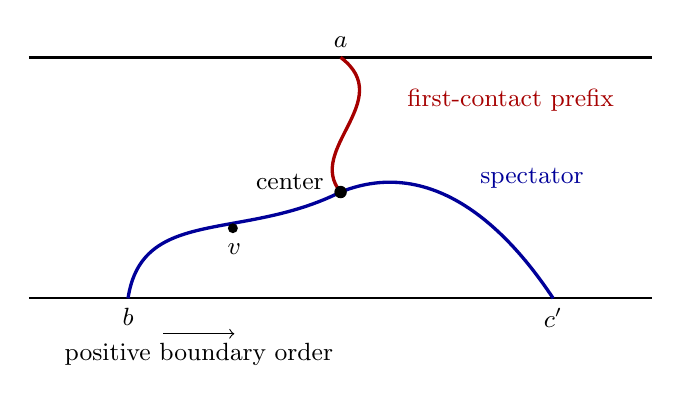
\begin{tikzpicture}[scale=.9, every node/.style={font=\small}]
 \draw[thick] (-.4,0)--(8.4,0);
 \draw[thick] (-.4,3.4)--(8.4,3.4);
 \node[below] at (1,0) {$b$};
 \node[below] at (7,0) {$c'$};
 \node[above] at (4,3.4) {$a$};
 \draw[very thick,blue!60!black] (1,0)
  .. controls (1.2,1.3) and (2.6,.8) .. (4,1.5);
 \draw[very thick,blue!60!black] (4,1.5)
  .. controls (5.5,2.1) and (6.6,.6) .. (7,0);
 \draw[very thick,red!65!black] (4,3.4)
  .. controls (4.8,2.8) and (3.5,2.1) .. (4,1.5);
 \fill (4,1.5) circle (2.5pt);
 \node[left] at (3.9,1.65) {center};
 \fill (2.48,.99) circle (2pt);
 \node[below] at (2.5,.91) {$v$};
 \node[blue!60!black] at (6.7,1.7) {spectator};
 \node[red!65!black] at (6.4,2.8) {first-contact prefix};
 \draw[->] (1.5,-.5)--(2.5,-.5);
 \node[below] at (2,-.5) {positive boundary order};
\end{tikzpicture}
\caption{A contact tripod, shown schematically. The arch from $b$ to
$c'$ is the spectator and a prefix from the opposite port $a$ reaches
it for the first time at the center. The center is weighted once.
Reassigning the active arm gives the two bridge-spectator terms.
The vertex $v$ may lie on any arm or at the center; the restrictions
in the proof keep these cases separate.}
\label{fig:pv:tripod}
\end{figure}


Let \(L_*\) sum all tripods containing \(v\), using the first (common) phase \(e^{i\sigma W_a}\).

The following sums use independent spectator and active paths, with
only the active path phased. A full exit includes all its visited
vertex weights; a prefix $\eta$ stops just before $v$ and omits its
weight. The port order and the sum over both choices of side are as
above.
\begin{center}
\small
\renewcommand{\arraystretch}{1.15}
\begin{tabular}{@{}p{.09\textwidth}p{.35\textwidth}p{.48\textwidth}@{}}
\toprule
Sum & Spectator & Active path and contact condition\\
\midrule
$A$ & Arch $b\to c'$ containing $v$
 & Full exit from $a$, hitting the spectator\\
$E_A$ & Arch $b\to c'$ avoiding $v$
 & Full exit from $a$, hitting both the spectator and $v$\\
$R_A$ & Arch $b\to c'$ avoiding $v$
 & Prefix $\eta$ from $a$, hitting the spectator before its stop\\
\midrule
$Z_b$ & Bridge $c'\to a$ containing $v$
 & Full exit from $b$, hitting the spectator\\
$Z_{c'}$ & Bridge $b\to a$ containing $v$
 & Full exit from $c'$, hitting the spectator\\
\midrule
$E_C$ & Bridge avoiding $v$, counted once
 & Full exit from any boundary source, hitting the spectator and $v$\\
$R_C$ & Bridge avoiding $v$, counted once
 & Prefix $\eta$ from any boundary source, hitting the spectator\\
\bottomrule
\end{tabular}
\end{center}
Set $Z=Z_b+Z_{c'}$. In $E_C$ and $R_C$, the active source may lie
on either boundary and may coincide with a spectator endpoint.

Hitting a marked spectator is represented by first contact by deletion. This gives exactly the contact tripod weights; in particular \(A,p Z_b,\bar p Z_{c'}\) in common phase restrict \(L_*\) to \(v\) not exclusively on the open arm \(a,b,c'\), respectively. The contact representation uses the free third edge for the incoming active prefix, since its source differs from the spectator endpoints. When the spectator avoids \(v\), the term in which \(v\) is visited before first contact is instead the complementary restriction in \(L_*\), with phase depending on the active arm. Thus
\[
 R_A=E_A+A-L_*,\qquad R_C=E_C+Z-2k L_*.
\]
This uses the both-obstacles formula above; if the active source coincides with a bridge spectator endpoint, all exits and prefixes to \(v\) hit that spectator with no possible \(v\) before first contact, consistent with the second equation.

For another balance, let the spectator now be a prefix $\eta$ from the
top weighted with \emph{conjugate} phase, and grow the opposite active
path in $S\setminus\{v\}$. Its valid ends are an original outer
boundary port or an attempt at $v$, stopped before taking its weight.
Revisit pairs from an outer source still cancel, with or without
deleting the spectator vertices. Use also the bottom spectator and top
active balance, add, and take real parts. The real sum of products for
valid leaves hitting those spectators is
\[
 \Re(2c R_A+R_C)+2P,\qquad
 P=\Re\!\!\sum_{\eta_B\cap\eta_T\ne\varnothing}
 w(\eta_B) w(\eta_T) e^{i\sigma(W_B-W_T)}
\]
where subscripts denote the lower/upper source and $w$ denotes absolute
path weight. Outer leaves are arches avoiding $v$ (both orientations,
averaging to phase $c$) or bridges avoiding $v$ (phase $1$); the other
leaves are the intersecting prefixes.

Write $u_B,u_T$ for the once-counted arch weights through $v$ on the
bottom and top, so $u=u_B+u_T$. By deletion, the two full prefix sums
are the nonnegative real numbers
\[
 M_B=m+2cu_B,\qquad M_T=m+2cu_T.
\]
Disjoint opposite-side prefixes join at $v$ to give each bridge through
$v$ once. Their product omits exactly the weight $x_*$ at $v$, and
their arrival-turn difference is $\pm\pi/3$, with real phase $k$.
Subtracting these disjoint pairs from the full product gives
\begin{equation}\label{eq:pv:prefix-product}
 P=M_BM_T-\frac{k}{x_*}m\ge-\frac{k}{x_*}m.
\end{equation}

At first contact the two shoulders from opposite sides form a bridge
$\lambda$ avoiding $v$. The incoming active edge is free: neither the
edge toward the spectator's source nor the edge toward its stopped-at
$v$ could have brought the opposite active path to its first contact.
The spectator suffix starts along the third edge from the center and
goes to $v$, avoiding $\lambda$. The bridge takes the center weight
once; the suffix takes neither that weight nor the weight at $v$.
Conversely these objects give all contacts once per choice of active
side.

Write $\delta=\pm\pi/3$ for the bottom-to-top join turn at the center,
and $W'$ for the suffix turn starting along its outgoing edge. The
shoulder-turn difference is $-\delta$; the turn into the suffix from
the top is $\delta$, and from the bottom $-\delta$. The two phase
factors therefore add to $2g e^{-i\sigma W'}$. For fixed $\lambda$,
the real suffix sum without $2g$ is exactly the real sum of prefixes
to $v$ in $S-\lambda$ from the new boundary ports on the unused
outward edges of $\lambda$. Length zero is included when appropriate.

Write $H(S;v)$ and $H(S-\lambda;v)$ for the real prefix sums to $v$
from the respective whole boundaries. Original prefixes avoiding
$\lambda$ are unchanged, so the new-boundary suffix sum equals the
original-boundary prefix sum hitting $\lambda$, minus
\[
 \Delta_\lambda=H(S;v)-H(S-\lambda;v)\ge0.
\]
For the inequality, reverse to exits from $v$ and use the positive
nesting expansion of Proposition~\ref{prop:pv:visits}, whose final
multipliers are $3+(2/x_*)\sum_Q c_{m_Q}w(Q)$. The domain $S-\lambda$
is filled: a removed bridge connected to the outer boundary cannot
enter the strict interior of a polygon avoiding it. For fixed
$\lambda$, take the nesting comparison first in convex lateral
truncations with and without its vertices, and then pass to the strip;
side contributions anchored at $v$ vanish by the convergence already
proved. When summing $w(\lambda)\Delta_\lambda$, use its representation
as hit prefixes minus new-boundary prefixes. Both are connected
terms; no sum of disconnected boundary terms is needed.
The first-contact calculation consequently gives
\[
 \Re(2cR_A+R_C)+2P=2g\left[\Re R_C-\sum_{\lambda\not\ni v}w(\lambda)\Delta_\lambda\right].
\]
Using the earlier equations (the \(L_*\) terms cancel since \(\phi k=c\)),
\[
 2c\Re(A+E_A)+2P\le \phi\Re(E_C+Z).
\]

\subsection{Comparison of intersecting path pairs}

We now compare the phased expressions with the positive pair sums.
Including only bridge exits as active paths gives $\Re(A+E_A)\ge J$;
the remaining exits have positive real weights. Also
$\Re(E_C+Z)\le2cJ+2J_{CC}$: allow active sources coinciding with a
marked spectator endpoint, adding nonnegative real weight, and combine
both orientations of every active path. Together with
\eqref{eq:pv:prefix-product}, the last phased inequality becomes
\[
 2c(1-\phi)J\le2\phi J_{CC}+\frac{2k}{x_*}m.
\]
Since $\phi<1$, this proves \eqref{eq:pv:pair-target}.

Let $\mu_h$ be the unnormalized measure on bottom-to-top bridge shapes
from one fixed bottom port, of total mass $b_h$. Write $X(\beta)$ for
the largest horizontal distance of a visited vertex from that source,
as in Lemma~\ref{lem:pv:lateral-tail}, and set $T=h\log^2h$ for large
$h$. If both bridge shapes have $X\le T$, then for any fixed marked
bridge the other shape has at most $CT$ translations hitting it.
Choosing which member contains $v$ only changes the constant. Thus
\[
 J_{CC}\le CTb_hm+R_h,
\]
where $R_h$ is the contribution of pairs with at least one $X>T$.

We bound this remainder absolutely, without an estimate on $m$.
A fixed-source shape $\beta_1$ has at most $|\beta_1|$ translations
placing a visited vertex at $v$, and
$|\beta_1|\le C(h+1)(X_1+1)$, where $X_i=X(\beta_i)$.
For each such translate, a second shape has at most
$C(X_1+X_2+1)$ translations hitting it. Hence, uniformly in $v$,
\begin{align*}
 R_h&\le C(h+1)
 \iint_{\max(X_1,X_2)>T}(1+X_1+X_2)^2
 \,d\mu_h(\beta_1)\,d\mu_h(\beta_2)\\
 &\le C(h+1)(T+h+1)^2e^{-cT/(h+1)}=O(h^{-100}).
\end{align*}
The second line follows by integrating the exponential tail in
Lemma~\ref{lem:pv:lateral-tail} for the first two moments of $X$,
using $b_h\le1$ and splitting according to which $X_i>T$.
Since $b_h=h^{-1/4+o(1)}$, we obtain
\begin{equation}\label{eq:pv:bridge-pair-upper}
 J_{CC}\le h^{3/4+o(1)}m+O(h^{-100}).
\end{equation}

\subsection{Translation hits on a deep arch}

The upper pair bound pays one bridge crossing mass for each allowed
horizontal translation. We need a matching lower bound for bridges
hitting each arch through the marked vertex. Here the error must be
uniform in the arch, whose length and horizontal span are unrestricted.

\begin{lemma}[Translated bridge hits]\label{lem:pv:translation-hits}
Let $\alpha$ be any same-side arch meeting the central third of the
strip. Let $\mathcal H_h(\alpha)$ be the total weight of strip bridges,
summed over all bottom sources, that intersect $\alpha$. For every
fixed $\epsilon\in(0,1)$,
\[
 \mathcal H_h(\alpha)\ge h^{3/4-\epsilon-o(1)},
\]
uniformly over all such arches. In particular
$\mathcal H_h(\alpha)\ge h^{3/4-o(1)}$ uniformly.
\end{lemma}

\begin{proof}
By reflection in the strip midline, it suffices to treat a bottom
arch. Translate its start to the fixed bottom source, put
$W=h^{1-\epsilon}$, and consider its prefix up to first crossing
layer $r=\lfloor h/4\rfloor$. Such a crossing exists because the arch
meets the central third.

\emph{Equal-height contact intervals.}
We first compare two prefixes $\alpha_0,\beta_0$ from the bottom to
their first crossings of the same cut. Parametrize them on $[0,1]$;
their heights lie strictly between the two cut heights internally.
There is a compact connected set of equal-height parameter pairs
containing $(0,0)$ and $(1,1)$, whose projections onto both parameter
intervals are all of $[0,1]$. Consequently its horizontal-difference
image is an interval of translations giving contact. It contains the
start and final offsets, and also an offset matching any prescribed
point on either prefix with a point on the other.

This is the piecewise-linear mountain-climbing construction
\cite[Theorem~5.5]{Pak2010}; we give the contact argument needed here.
On the parameter square, triangulate so that the height difference is
piecewise linear. For sufficiently small positive regular values its
level set has exactly two boundary endpoints, near the diagonal
corners, joined by an arc. Indeed the two prefix heights are strictly
monotone near their extremal endpoints and stay away from these
extremal heights on every compact interior parameter interval.
A subsequential Hausdorff limit of the compact arcs is connected,
lies in the zero set, and contains both corners. Such a subsequence
can also be obtained by diagonal selection of the dyadic boxes met by
the arcs. Each coordinate projection is connected and contains $0$
and $1$, hence equals $[0,1]$. Taking horizontal differences proves
the interval assertion. At integer translations, geometric contact
of the lattice walks gives a shared vertex. A contact at the
intermediate cut is also a shared vertex of the full walks, since
that port lies inside their lattice edges.

\emph{Two direct alternatives.}
Suppose first that at some intermediate cut the arch prefix has two
crossings at horizontal distance at least $W$. Every bridge shape
then has at least $W-O(1)$ hitting translates. To see this, use the
bridge crosscut's left/right side indicator at the two points, with
any fixed convention for points on it. Their separation is an integer.
Summing the signed indicator difference over integer translates
telescopes to that integer in absolute value. Any discrepancy forces
the intervening arch segment to meet the bridge. Summing bridge
shapes therefore gives hitting mass at least $(W-O(1))b_h$.

Suppose next that the arch's displacement $a$ at first crossing of
some layer $1,\ldots,r$ satisfies $|a|\ge W$. A bridge and its
reflection about its start have first-crossing displacements $d$ and
$-d$ there, and
\[
 \max\{|a-d|,|a+d|\}\ge |a|\ge W.
\]
For at least one member of this reflection pair, the contact interval
between the start and final offsets yields $W-O(1)$ hitting
translates. Reflection preserves weights, so again the hitting mass
is at least a constant times $Wb_h$.

In the remaining case every first-crossing displacement is less than
$W$ and every same-cut crossing spread is less than $W$. Thus all
cut crossings of the arch prefix lie within $2W$ of its start.
The full prefix stays within $2W+O(1)$: inside a cut-to-cut layer a
walk between ports follows the internal zigzag monotonically.

\emph{Wide bridge prefixes against a confined arch.}
We will show that fixed-source bridges of weight at least
$h^{-1/4-o(1)}$ make lateral distance greater than $4W$ before their
first crossing of layer $r$. We first bound the exceptional confined
pieces that enter the marking argument.

For $h/10\le j\le h/6$, let $e_j$ be the weight of fixed-source
$j$-bridges confined to lateral distance $4W$ from their start. Then
\begin{equation}\label{eq:pv:tube-exception}
 e_j\le C\exp(-ch/W).
\end{equation}
Surround the width-$8W$ tube by a tube of width $O(W)$ whose side
walls alternate the two slanted upward tiling steps between successive
horizontal layers, outside the desired confinement with a safety
margin. Join these walls horizontally on top and bottom. Starting
east along the positive bottom boundary, its unwrapped tangent
angles stay in $[0,2\pi]$: on the right wall they are
$\pi/3,2\pi/3$, and on the left $4\pi/3,5\pi/3$. For a bottom
source, closing an exit by the boundary gives turn $B-\pi$, where
$B\in[0,2\pi]$ is the cumulative tangent turn from source to exit.
Thus all original exits have turns in $[-\pi,\pi]$ and positive
comparable real weights. This supplies the needed positivity even
though the tube is not convex.

Now cut by lines with the two slanted upward normals, of angles
$\pm\pi/3$ from vertical. Boundary-source leaf cancellation still
holds after either cut, since a polygon cannot surround the bottom
source. The genuinely new exits lie on the cut and stay in the convex
wedge between its half-plane and the half-plane above the bottom,
so their turns are fixed. The lost exit sums consequently lie on two
separated rays. Place the intercepts at the source's lateral
coordinate near $s+C'(W+1)$, stagger them by $O(W+1)$, and round to
tiling lines. Since all lateral coordinates are restricted to
$O(W+1)$, the two lost events are nested between reaching heights
$s+C(W+1)$ and $s$. The separated-ray argument of
Lemma~\ref{lem:pv:lateral-tail}, with the positive original exit
weights just established, gives fixed-factor decay per such height
increment, starting at $O(W+1)$. The confined $j$-bridges are among
the top exits of this tube. This proves
\eqref{eq:pv:tube-exception}.

Under the fixed-source bridge measure $\mu_h$ defined above, let
$N(\gamma)$ count layers
$j\in[\lceil h/10\rceil,\lfloor h/6\rfloor]$ that it crosses
exactly once and whose initial $j$-bridge reaches lateral distance
greater than $4W$. At a single-crossing cut, the two bridge pieces
occupy disjoint open slabs. Their weights multiply exactly, since
ports carry no weight. Proposition~\ref{prop:pv:boundary} and
\eqref{eq:pv:tube-exception} give
\begin{align*}
 \int N\,d\mu_h
 &=\sum_j b_{h-j}(b_j-e_j)=h^{1/2+o(1)},\\
 \int N^2\,d\mu_h
 &\le2\sum_{j_1\le j_2}
 b_{j_1}b_{j_2-j_1}b_{h-j_2}
 \le h^{5/4+o(1)}.
\end{align*}
For the second line, dropping the lateral excursion restrictions
leaves three bridge pieces. Use $b_0=1$ on the diagonal and
$\sum_{d\le h}b_d=h^{3/4+o(1)}$; the two outside factors each have
order $h^{-1/4+o(1)}$, uniformly over the chosen layers. Hence
unnormalized Cauchy--Schwarz yields
\[
 \mu_h(N>0)\ge
 \frac{\big(\int N\,d\mu_h\big)^2}{\int N^2\,d\mu_h}
 \ge h^{-1/4-o(1)}.
\]
Every bridge counted here has the required lateral excursion before
first crossing $r$. Apply the contact-interval construction to the
two prefixes ending at $r$, matching that prescribed excursion point
of the bridge to the confined arch prefix. The resulting offset
differs from the initial offset by at least $2W-O(1)$, and hence gives
at least order $W$ integer hitting translates. Their total weight is
at least $W h^{-1/4-o(1)}=h^{3/4-\epsilon-o(1)}$.

All three alternatives give this bound with constants and errors
independent of the arch. For each fixed $\epsilon$, first let
$h\to\infty$; only then let $\epsilon\downarrow0$. This proves the
uniform exponent assertion.
\end{proof}

\subsection{The bridge first moment}

Lemma~\ref{lem:pv:translation-hits} gives
$J\ge h^{3/4-o(1)}u$. Combining this with
\eqref{eq:pv:pair-target} and \eqref{eq:pv:bridge-pair-upper} yields
\[
 u\le h^{o(1)}m+O\big(h^{-100-3/4+o(1)}\big).
\]
On the other hand, $2(u+m)=A_{S_h}(v)$: the ordered excursion
convention counts each path twice. Lemma~\ref{lem:pv:strip-visits}
therefore gives $u+m=h^{1/12+o(1)}$ in the central third, uniformly
in $v$. The negligible additive error above cannot carry this mass,
so
\begin{align*}
 m(v)&=h^{1/12+o(1)}
 &&\text{uniformly in the central third},\\
 m(v)&\le h^{1/12+o(1)}
 &&\text{throughout the strip}.
\end{align*}

To pass from a marked vertex to a fixed source, let $\mathcal V_h$
contain one representative of each horizontal-translation orbit of
strip vertices. Translating a bridge's bottom source to the fixed
source identifies $m(v)$ with the weighted number of visits to the
orbit of $v$. Thus the unnormalized fixed-source length mass is
exactly
\[
 \ell_h=\sum_{v\in\mathcal V_h}m(v).
\]
There are $O(h)$ such orbits, with order $h$ represented in the
central third. The pointwise upper and lower estimates give
$\ell_h=h^{13/12+o(1)}$. Finally, dividing by
$b_h=h^{-1/4+o(1)}$ gives
\[
 \mathbb E|\gamma|=\frac{\ell_h}{b_h}=h^{4/3+o(1)}.
\]
Lemma~\ref{lem:pv:lateral-tail} makes both the discarded mass and
discarded first moment at horizontal range $h\log^2h$ negligible,
so the same conclusion holds with that confinement. This completes
Theorem~\ref{thm:pv:bridge}.
